\hypertarget{collective-communication-in-distributed-memory-systems}{%
\section{Collective Communication in Distributed-Memory
Systems}\label{collective-communication-in-distributed-memory-systems}}

\begin{itemize}
\tightlist
\item
  designing parallel algorithms on a distributed-memory system requires
  data exchange between processes (nodes)
\item
  this exchange can significantly impact the efficiency because of
  interaction delays
\end{itemize}

\hypertarget{communication-costs}{%
\subsection{Communication Costs}\label{communication-costs}}

\begin{itemize}
\tightlist
\item
  Overhead in parallel programs

  \begin{itemize}
  \tightlist
  \item
    idling
  \item
    contention
  \item
    communication
  \end{itemize}
\item
  Communication costs depend on

  \begin{itemize}
  \tightlist
  \item
    communication model
  \item
    the network topology
  \item
    data handling and routing (e.g.~packet routing, cut-through routing)
  \item
    associated software protocols
  \end{itemize}
\end{itemize}

The message passing costs is the total time to transfer a message over a
network and is comprised of the following:

\begin{itemize}
\tightlist
\item
  Startup time ($t_s$)

  \begin{itemize}
  \tightlist
  \item
    executing the routing algorithm, programming routers, etc.
  \end{itemize}
\item
  Per-hop time ($t_h$)
\item
  Per-word transfer time ($t_w$)
\item
  $t_h$ is typically smaller than $t_s$ and $t_w$ , so the second term does
  not show, when $m$ is large
\item
  furthermore, it is often not possible to control routing and placement
  of tasks
\end{itemize}

\begin{figure}[H]
\centering
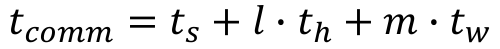
\includegraphics[width=0.4\textwidth]{figures/communicationCosts.png}
\caption{Communication costs}
\end{figure}

\begin{tcolorbox}[colback=red!5!white,colframe=red!75!black]
The simplified cost model: $t_{comm} = t_s + m * t_w$
\end{tcolorbox}

\hypertarget{introduction-to-collective-communication}{%
\subsection{Introduction to Collective
Communication}\label{introduction-to-collective-communication}}

\begin{figure}[H]
\centering
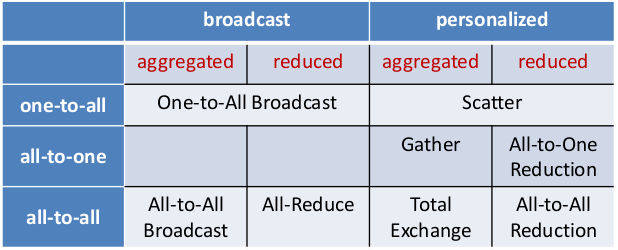
\includegraphics[width=0.5\textwidth]{figures/globalCommunication.png}
\caption{Overview Global Communication}
\end{figure}

\hypertarget{one-to-all-broadcast-and-all-to-one-reduction}{%
\subsection{One-to-All Broadcast and All-to-One
Reduction}\label{one-to-all-broadcast-and-all-to-one-reduction}}

\begin{itemize}
\tightlist
\item
  One-to-All Broadcast

  \begin{itemize}
  \tightlist
  \item
    one processor has a message M (of size m) it needs to send to
    everyone
  \end{itemize}
\item
  All-to-One Reduction

  \begin{itemize}
  \tightlist
  \item
    the dual of one-to-all broadcast
  \item
    each processor has m units of data
  \item
    these data items must be combined piece-wise (using some associative
    operator, such as addition or min for example)
  \item
    the result made available at a target node
  \end{itemize}
\end{itemize}

\hypertarget{one-to-all-broadcast-on-a-ring}{%
\subsubsection{One-to-All Broadcast on a
Ring}\label{one-to-all-broadcast-on-a-ring}}

\begin{figure}[H]
\centering
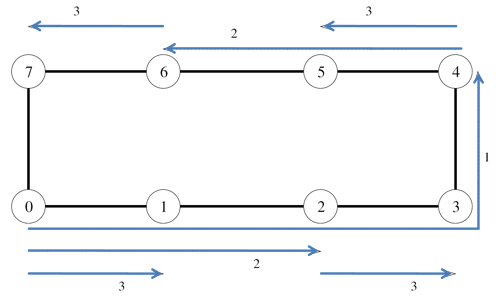
\includegraphics[width=0.5\textwidth]{figures/one-to-all-broadcast.png}
\caption{One-to-All Broadcast}
\end{figure}

\begin{itemize}
\tightlist
\item
  node 0 is the source of the broadcast
\item
  each message transfer step is shown by an arrow from the source of the
  message to its destination
\item
  the number on an arrow indicates the time step during which the
  message is transferred
\end{itemize}

\hypertarget{all-to-one-reduction-on-a-ring}{%
\subsubsection{All-to-One Reduction on a
Ring}\label{all-to-one-reduction-on-a-ring}}

\begin{figure}[H]
\centering
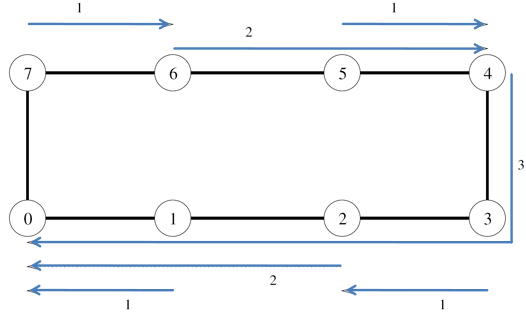
\includegraphics[width=0.5\textwidth]{figures/all-to-one-reduction-ring.png}
\caption{All-to-One Reduction}
\end{figure}

\hypertarget{broadcast-and-reduction-algorithms}{%
\subsubsection{Broadcast and Reduction
Algorithms}\label{broadcast-and-reduction-algorithms}}

\begin{itemize}
\tightlist
\item
  These algorithms can also be used in a mash of p nodes

  \begin{itemize}
  \tightlist
  \item
    the first step does the operation along a row
  \item
    the second step along each column concurrently
  \end{itemize}
\item
  this process generalizes to higher dimensions as well

  \begin{itemize}
  \tightlist
  \item
    e.g.~a hypercube with $2^d$ nodes can be regarded as a d-D mesh with
    two nodes in each dimension
  \end{itemize}
\end{itemize}

\hypertarget{all-to-all-broadcast-and-reduction}{%
\subsection{All-to-All Broadcast and
Reduction}\label{all-to-all-broadcast-and-reduction}}

\begin{itemize}
\tightlist
\item
  Broadcast

  \begin{itemize}
  \tightlist
  \item
    Generalization of broadcast in which each node is the source as well
    as the destination
  \item
    A node sends the same m-word message to every other node, but
    different nodes may broadcast different messages
  \end{itemize}
\item
  Reduction

  \begin{itemize}
  \tightlist
  \item
    every node is the destination of an all-to-one reduction
  \item
    each node starts with p messages
  \end{itemize}
\end{itemize}

\hypertarget{all-to-all-broadcast-in-a-ring}{%
\subsubsection{All-to-All Broadcast in a
Ring}\label{all-to-all-broadcast-in-a-ring}}

\begin{figure}[H]
\centering
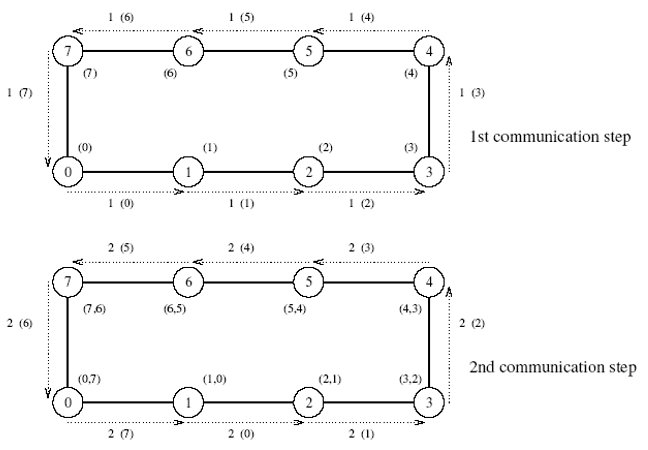
\includegraphics[width=0.7\textwidth]{figures/all-to-all-broadcast.png}
\caption{All-to-All Broadcast Ring}
\end{figure}

\begin{itemize}
\tightlist
\item
  each node first sends to one of its neighbors the data it needs to
  broadcast
\item
  in subsequent steps, it forwards the data received from one of its
  neighbors to its other neighbor
\item
  the algorithm terminates in p-1 steps
\item
  \textbf{Reduction} can be performed in an identical fashion by
  inverting the process
\end{itemize}

\hypertarget{all-to-all-broadcast-on-a-mesh}{%
\subsubsection{All-to-All Broadcast on a
Mesh}\label{all-to-all-broadcast-on-a-mesh}}

\begin{figure}[H]
\centering
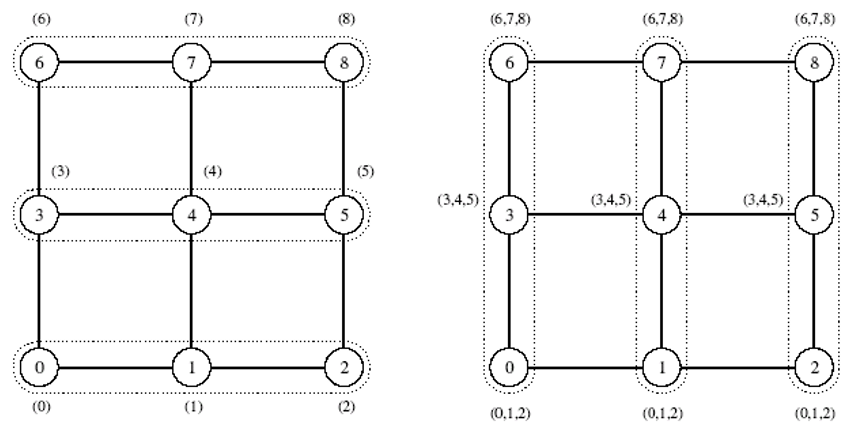
\includegraphics[width=0.5\textwidth]{figures/all-to-all-broadcast-mesh.png}
\caption{All-to-All Broadcast Mesh}
\end{figure}

\begin{itemize}
\tightlist
\item
  each row of the mesh performs an all-to-all broadcast using the
  procedure for the linear array
\item
  in this phase, all nodes collect sqr(p) messages corresponding to the
  sqr(p) nodes of their respective rows
\item
  each node consolidates this information into a single message of size
  m * sqr(p)
\end{itemize}

\clearpage
\hypertarget{all-reduce}{%
\subsection{All-Reduce}\label{all-reduce}}

Each node starts with a buffer of size m and the final results of the
operation are identical buffers of size m on each node that are formed
by combining the original p buffers using an associative operator.

\begin{itemize}
\tightlist
\item
  inefficient approach

  \begin{itemize}
  \tightlist
  \item
    identical to all-to-one reduction followed by a one-to-all broadcast
  \end{itemize}
\item
  better approach

  \begin{itemize}
  \tightlist
  \item
    uses the pattern of all-to-all broadcast, but without increasing
    message size
  \item
    hypercube: $T = (t_s + mt_w) * log(p)$
  \end{itemize}
\end{itemize}

\hypertarget{scatter-and-gather}{%
\subsection{Scatter and Gather}\label{scatter-and-gather}}

\begin{itemize}
\tightlist
\item
  Scatter

  \begin{itemize}
  \tightlist
  \item
    a single node sends a unique message of size m to every other node
    (also called a one-to-all personalized communication)
  \item
    is fundamentally different from broadcast
  \item
    but the algorithmic structure is similar
  \end{itemize}
\item
  Gather

  \begin{itemize}
  \tightlist
  \item
    a single node collects a unique message from each node
  \item
    the gather operation is exactly the inverse of the scatter operation
    and can be frexecuted as such
  \end{itemize}
\end{itemize}

\hypertarget{all-to-all-personalized-communication-total-exchange}{%
\subsubsection{All-to-All Personalized Communication (Total
Exchange)}\label{all-to-all-personalized-communication-total-exchange}}

\begin{itemize}
\tightlist
\item
  each node has a distinct message of size m for every other node
\item
  this is unlike all-to-all broadcast, in which each node sends the same
  message to all other nodes
\end{itemize}

\clearpage
\hypertarget{all-to-all-personalize-communication-on-a-ring}{%
\subsubsection{All-to-All Personalize Communication on a
Ring}\label{all-to-all-personalize-communication-on-a-ring}}

\begin{itemize}
\tightlist
\item
  each node sends all pieces of data as one consolidated message of size
  m(p -- 1) to one of its neighbors
\item
  each node extracts the information meant for it from the data
  received, and forwards the remaining pieces of size m each to the next
  node
\item
  the size of the consolidated message reduces by m at each step
\end{itemize}

\begin{figure}[H]
\centering
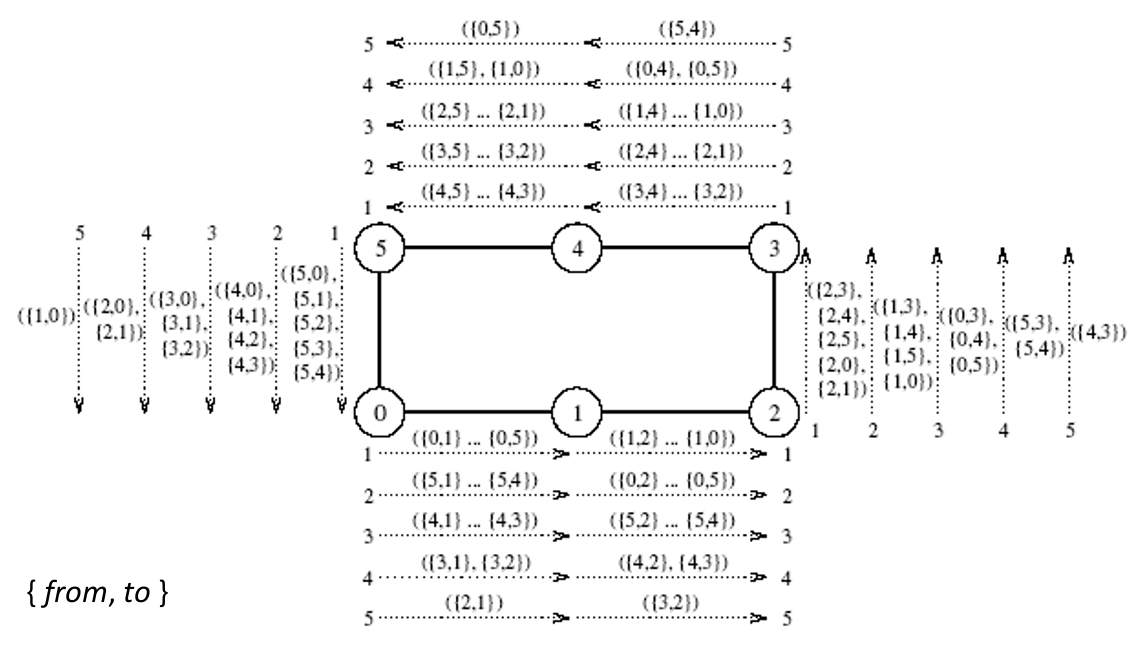
\includegraphics[width=0.7\textwidth]{figures/all-to-all-ring.png}
\caption{All-to-All Ring}
\end{figure}

\hypertarget{summary-of-communication-times}{%
\subsection{Summary of communication
times}\label{summary-of-communication-times}}

\begin{figure}[H]
\centering
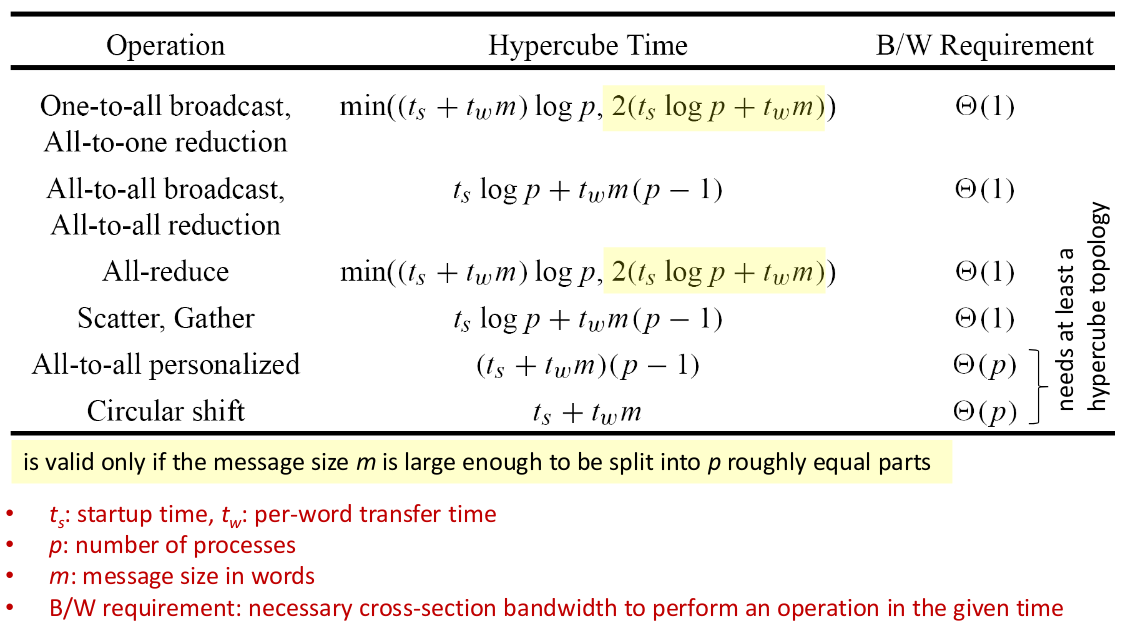
\includegraphics[width=0.8\textwidth]{figures/summary-CommunicationTimes.png}
\caption{Summary of all communication times}
\end{figure}

\clearpage